% Research theme figure: Multiphysics Fluid Flow
% (coupled physics -> MHD convection -> phase change). Same canvas, fonts and palette
% as the other research figures; greyscale on the site, colour on hover.
% Build (from this folder):
%   latex multiphysics.tex
%   dvisvgm --no-fonts --bbox=papersize -o ../multiphysics.svg multiphysics.dvi
\def\pgfsysdriver{pgfsys-dvisvgm.def}
\documentclass[tikz,border=0pt]{standalone}
\usetikzlibrary{arrows.meta}
\renewcommand{\familydefault}{\sfdefault}

% --- palette (shared with the other research figures) ------------------------
\definecolor{ink}{HTML}{1A1A1A}
\definecolor{frame}{HTML}{4D4D4D}
\definecolor{steel}{HTML}{245A94}
\definecolor{sky}{HTML}{6E9FD2}
\definecolor{mist}{HTML}{D3E3F3}
\definecolor{amber}{HTML}{C8702A}
\definecolor{sand}{HTML}{F0CFA8}

\begin{document}
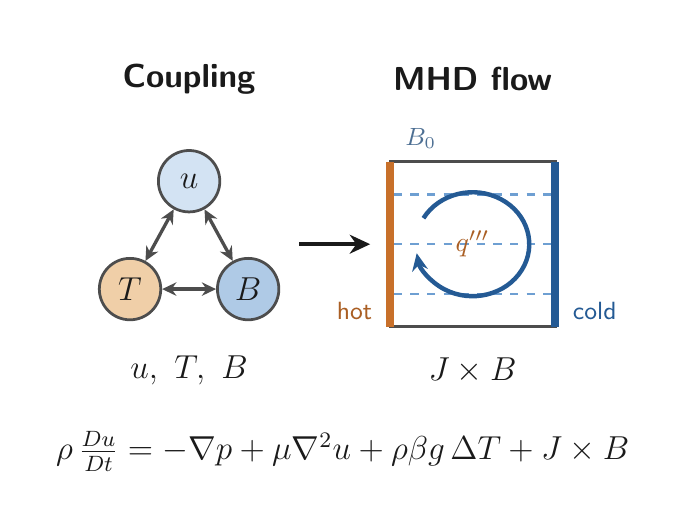
\begin{tikzpicture}[
    line width=1.6pt, >={Stealth[length=2.6mm,width=2.4mm]},
    small arrow/.style={-{Stealth[length=1.8mm,width=1.7mm]}, line width=1.2pt},
    both arrow/.style={{Stealth[length=1.8mm,width=1.7mm]}-{Stealth[length=1.8mm,width=1.7mm]}, line width=1.2pt},
    color=ink,
    title/.style={font=\large\bfseries, text=ink},
    lab/.style={font=\large, text=ink},
    field/.style={circle, draw=frame, line width=1.0pt, minimum size=0.78cm, inner sep=0pt, font=\large, text=ink}]
  % fixed 8 cm x 6 cm canvas
  \path[use as bounding box] (0,0) rectangle (8,6);

  % ================= 1) coupled physics =================
  \node[title] at (2.05,5.35) {Coupling};
  \node[field, fill=mist] (u) at (2.05,4.05) {$u$};
  \node[field, fill=sand] (T) at (1.30,2.68) {$T$};
  \node[field, fill=sky!55] (B) at (2.80,2.68) {$B$};
  \draw[both arrow, frame] (u) -- (T);
  \draw[both arrow, frame] (u) -- (B);
  \draw[both arrow, frame] (T) -- (B);
  \node[lab] at (2.05,1.65) {$u,\ T,\ B$};

  % ================= 2) MHD natural convection in a cavity =================
  \node[title] at (5.65,5.35) {MHD flow};
  \fill[white] (4.60,2.20) rectangle (6.70,4.30);
  % applied magnetic field B0 (horizontal field lines)
  \foreach \y in {2.62,3.25,3.88}
    \draw[sky, line width=0.9pt, dashed] (4.65,\y) -- (6.65,\y);
  % convection roll (rises at the hot wall)
  \draw[steel, line width=1.6pt, -{Stealth[length=2.2mm,width=2.0mm]}]
    (5.65,3.25) ++(150:0.72 and 0.66) arc[start angle=150, end angle=-170, x radius=0.72, y radius=0.66];
  % internal heat generation
  \node[font=\normalsize, text=amber!85!black] at (5.65,3.25) {$q'''$};
  % walls: hot (left), cold (right), adiabatic (top, bottom)
  \draw[frame, line width=1.0pt] (4.60,2.20) rectangle (6.70,4.30);
  \draw[amber, line width=3.0pt] (4.60,2.20) -- (4.60,4.30);
  \draw[steel, line width=3.0pt] (6.70,2.20) -- (6.70,4.30);
  \node[font=\small, text=sky!70!black, anchor=south west] at (4.65,4.32) {$B_0$};
  \node[font=\small, text=amber!85!black, anchor=east] at (4.52,2.40) {hot};
  \node[font=\small, text=steel, anchor=west] at (6.78,2.40) {cold};
  \node[lab] at (5.65,1.65) {$J \times B$};

  % ================= arrow between panels =================
  \draw[->] (3.45,3.25) -- (4.35,3.25);

  % ================= momentum balance with buoyancy and Lorentz force =================
  \node[font=\large, text=ink] at (4.00,0.62)
    {$\rho\,\frac{Du}{Dt} = -\nabla p + \mu\nabla^2 u + \rho\beta g\,\Delta T + J\times B$};
\end{tikzpicture}
\end{document}
